\documentclass[letterpaper, oneside, 12pt,these,creativecommons]{thETS} 
\usepackage{times}
\usepackage[pdftex]{graphicx}
\usepackage{multirow}
\usepackage{pdfpages}
\usepackage{amsmath}
\usepackage{amssymb}
\usepackage{caption}
\usepackage[utf8]{inputenc}
\usepackage[frenchb]{babel}
\usepackage{amsmath}
\usepackage{caption}

\usepackage{glossaries}

\usepackage[round]{natbibETS} %Pour faire les citations du genre Autheur (Année)
\usepackage{multibib} %Pour faire la liste des références
\newcites{refs}{LISTE DE REFERENCES}
\usepackage{url} % Prise en charge des url pour les référence
\urlstyle{rm} % Hyphenation des références

\makeglossaries

\newglossaryentry{computer}
{
  name=computer,
  description={is a programmable machine that receives input,
               stores and manipulates data, and provides
               output in a useful format}
}


\listfiles

\diplome{
DU\\
B.A.C EN GENIE
}

\title{LOG350}
\author{Marc-André DESTREMPES\\Martin DESHARNAIS\\Simon GRONDIN}

\authorcopyright{}
\datesoutenance{``Date a venir''}
\datedepot{19 novembre 2012}
\directeur{M. }{Prenom Nom}{Nom du departement et institution}
%\codirecteur{Mme.}{Prenom Nom}{departement et institution}
\president{M.}{Prenom Nom}{departement et institution}
\examinexterne{M.}{Prenom Nom}{departement et institution}{}
\jury{Mme.}{Prenom Nom}{departement et institution}{}

\begin{document}

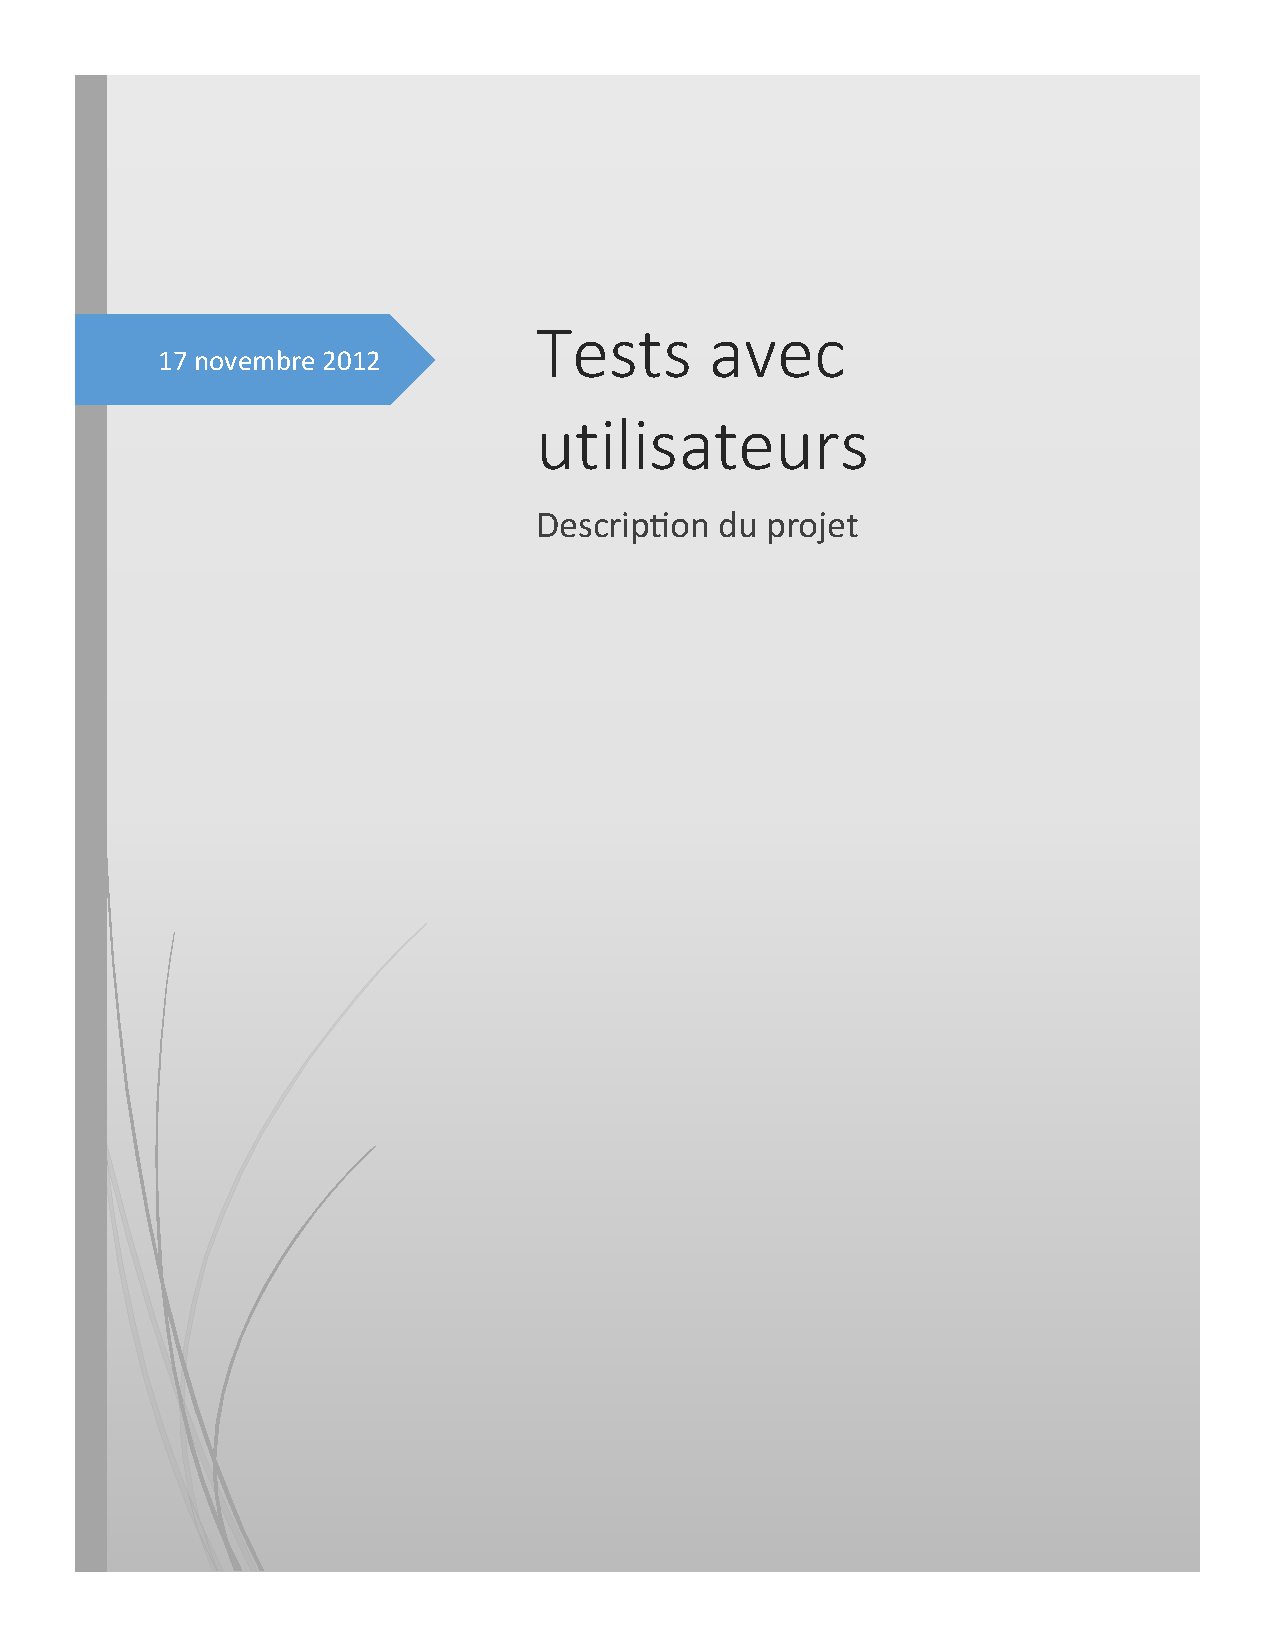
\includepdf[pages={1}]{PageTitre.pdf}

%\maketitle

\tableofcontents

\listoftables

%\listoffigures

\chapter{Contenu du document}

Le présent document contient une présentation sommaire du projet, une description de l'évaluation dont les méthodologies utilisées, le déroulement de l'évaluation ainsi qu'un exemple des fiches qui seront utilisées durant l'évaluation.

Ce document se veut à but descriptif pour que les utilisateurs comprennent bien le but de l'évaluation et le but premier du programme avant que ceux-ci le teste.

\chapter{Glossaire}

\begin{description}
\item [Tâche] Travail à effectuer
\item [Échéance] Date limite pour effectuer un travail
\item [Alerte] Rappel avant une date
\item [Événement] Activité, occurrence à une date donnée
\end{description}

\glsaddall
\printglossaries

\chapter{Présentation de l'application}

\section{Description de l'application}

L’application permettra la gestion de listes de taches et d’événements avec un niveau de priorité que l’utilisateur pourra lui assigner pour déterminer son importance et des alertes (rappels). Un système de tri avancé aide à trouver rapidement ce que l’on cherche. 

Un exemple d’utilisation complet serait le suivant:
L’utilisateur regarde les tâches qu’il a à faire pour la journée et les événements prévus. Il ajoute ensuite une tâche et lui assigne une sous-tâche. Il crée ensuite un événement et lui lie la tâche pour indiquer qu’elle est due à cette date.

\section{Contexte du domaine d’application et motivation}

Dans tous les domaines, les gens ont toujours eu besoin de quelque chose pour garder une trace de ce qu'ils ont à faire. Pour ce faire, ils utilisent divers outils comme un agenda, Microsoft Project, Trac, des post-it ou bien une simple liste. Pour répondre à ce besoin, nous avons décidé de développer un outil léger et efficace qui permet d'offrir une gestion des tâches et événements. Avec cet outil, il sera donc possible d'effectuer un suivi des choses à faire et des événements et de les classer comme bon nous semble. Par exemple, les gens aiment classer leurs choses par sujet, ce qui motive une interface pour visualiser les taches à effectuer et les événements par thème.

\section{Description du public cible et des types d’intervenants}

L'utilisateur cible est une personne de 15 ans et plus, cherchant à organiser son temps et sa vie professionnelle. Cette personne possède un ordinateur et connaît les rudiments de base de l’informatique.

Il n’y a qu’un seul intervenant, l’utilisateur lui-même. Il n’y a pas de mode multiutilisateurs.

\chapter{Description de l'évaluation}

\section{Méthodologies utilisées}

Les tests effectués seront les suivants : 
\begin{description}
\item [psychomoteurs] \hfill \\ relatif aux fonctions psychiques et motrices \footnote{\url{http://dictionnaire.reverso.net/francais-definition/psychomoteur}}
\item [de performance] \hfill \\ test dont l'objectif est de déterminer la performance d'un système informatique \footnote{\url{https://fr.wikipedia.org/wiki/Test_de_performance}}
\item [d’usabilité (tests, enquêtes et focus groups)] \hfill \\ consiste à observer directement l'utilisateur en train de se servir de l'application \footnote{\url{http://www.usabilis.com/methode/test-utilisateur.htm}}
\end{description}

\section{Déroulement de l'évaluation}

L'évaluateur prendra place avec l'utilisateur et lui dictera les actions que celui-ci devra effectuer. Lors de chaque opération l'évaluateur prendra des notes quand aux tests énumérés ci-dessus. De plus, l'utilisateur pourra donner son point de vue sur des améliorations possibles ou bien critiquer les défauts que celui-ci voit dans l'application.

\section{Exemple}

\subsection{Fiche de tâches à effectuer}

Cette fiche contient les tâches que l'évaluateur demandera à l'utilisateur d'effectuer.

\begin{table}[H]
\centering
\begin{tabular}{|l|l|l|}
	\hline
	no Tâche & Titre et description & Éléments que vous voulez vérifier et hypothèses \\ \hline
	1 & Ajouter une tâche en utilisant & L'utilisation des raccourcis disponible pour \\ 
	   & la barre d'ajout rapide. &  l'utilisateur. \\ \hline
	\dots & \dots & \dots \\ \hline
\end{tabular}
\caption{Tâches à effectuer}
\end{table}

\newpage

\subsection{Fiche de discussion et recommandation}

C'est dans cette fiche que l'évaluateur noteras les observations effectuées sur l'utilisateur et les recommandations que l'utilisateur mentionne à l'évaluateur.

\begin{table}[H]
\centering
\begin{tabular}{|l|l|l|}
	\hline
	no Tâche & Points importants de l’observation de A & Recommandations \\ \hline
	1 & L'utilisateur ne trouve pas comment & Rendre l'option plus visible et \\ 
	   & ajouter. & intuitive. \\ \hline
	\dots & \dots & \dots \\ \hline
\end{tabular}
\caption{Discussion et recommandation}
\end{table}

\end{document}